% !Mode:: "TeX:UTF-8"
% !TEX program  = xelatex
\section{Question 1}
\begin{statebox}{}{question-1}
    Modify the code to deal with a put option.
\end{statebox}
\Python{Put option}{code/9-10/lect9_put.m}
\Python{Geeks}{code/9-10/geeks.m}
\begin{figure}[H]
    \centering
    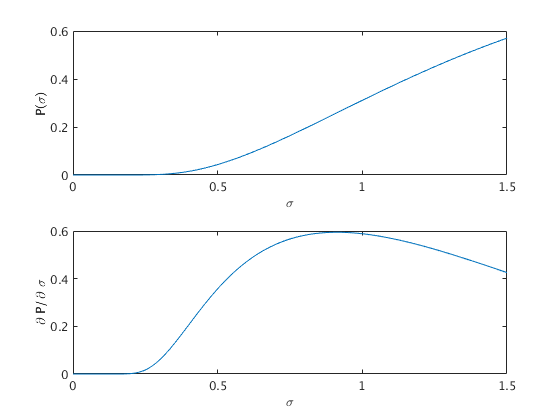
\includegraphics[width=.7\textwidth]{figures/2019-12-04-put.png}
    \caption{Put option}\label{F:1}
\end{figure}


\section{Question 2}
\begin{statebox}{}{question-2}
    Acquire some Geeks data, and create a figure as before. If possible, investigate the behavior of the implied volatility as the expiry time varies.
\end{statebox}
% Please add the following required packages to your document preamble:
% \usepackage{booktabs}
% 
% If you use beamer only pass "xcolor=table" option, i.e. \documentclass[xcolor=table]{beamer}
\begin{table}[H]
    \begin{tabular}{@{}lll@{}}
    \toprule
    Option Price & Exercise Price & Implied Volatility \\ \midrule
    0.2536       & 2.2            & 0.281              \\
    0.2075       & 2.25           & 0.2643             \\
    0.1664       & 2.3            & 0.2646             \\
    0.1267       & 2.35           & 0.2524             \\
    0.0954       & 2.4            & 0.2563             \\
    0.0679       & 2.45           & 0.2533             \\
    0.0468       & 2.5            & 0.2531             \\
    0.0315       & 2.55           & 0.2533             \\
    0.02         & 2.6            & 0.2548             \\
    0.0122       & 2.65           & 0.2545             \\
    0.007        & 2.7            & 0.2545             \\
    0.0042       & 2.75           & 0.2566             \\
    0.0028       & 2.8            & 0.266              \\
    0.0019       & 2.85           & 0.2753             \\
    0.0014       & 2.9            & 0.2875             \\
    0.0015       & 2.95           & 0.315              \\ \bottomrule
    \end{tabular}
\end{table}
\begin{figure}[H]
    \centering
    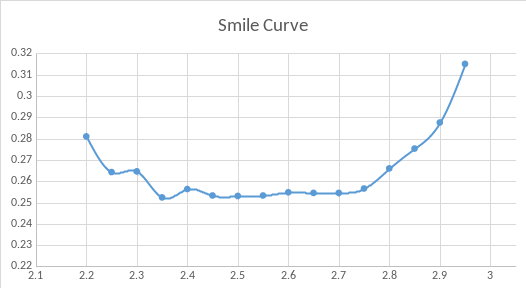
\includegraphics[width=.7\textwidth]{figures/2019-12-04-smile.png}
    \caption{Put option}\label{F:1}
\end{figure}
